\documentclass[11pt,a4paper]{article}
\usepackage[utf8]{inputenc}
\usepackage[T1]{fontenc}
\usepackage{geometry}
\geometry{top=2.5cm, bottom=2cm, left=2cm, right=2cm, headheight=15pt}
\usepackage{lmodern}
\usepackage{xcolor}
\usepackage{graphicx}
\usepackage{float}
\usepackage{hyperref}
\usepackage{enumitem}
\usepackage{booktabs}
\usepackage{tcolorbox}
\tcbuselibrary{skins, breakable}
\usepackage{titlesec}
\usepackage{fancyhdr}
\usepackage{colortbl}
\usepackage{longtable}

% Colors setup
\definecolor{sintefblue}{HTML}{1F5F74}
\definecolor{sintefgold}{HTML}{F4B942}
\definecolor{sintefred}{HTML}{E05A47}
\definecolor{darkgray}{HTML}{333333}
\definecolor{lightgray}{HTML}{F8F9FA}
\definecolor{headergray}{HTML}{EAECEE}

% Hyperref setup
\hypersetup{
    colorlinks=true,
    linkcolor=sintefblue,
    urlcolor=sintefblue,
    pdftitle={Cahier des Charges - Mini-Projet Data Mining 2026/2027},
    pdfauthor={Data Mining Course}
}

% Header and Footer setup
\pagestyle{fancy}
\fancyhf{}
\lhead{\color{sintefblue}\bfseries Data Mining — Mini-Projet}
\rhead{\color{sintefblue}Année Académique 2026/2027}
\lfoot{\small Cours de Data Mining}
\rfoot{\small Page \thepage}
\renewcommand{\headrulewidth}{0.8pt}
\renewcommand{\footrulewidth}{0.4pt}

% Section styling
\titleformat{\section}{\color{sintefblue}\Large\bfseries}{\thesection.}{0.5em}{}[\titlerule]
\titleformat{\subsection}{\color{sintefblue}\large\bfseries}{\thesubsection.}{0.5em}{}

\begin{document}

% Title Header Block
\begin{tcolorbox}[colback=sintefblue, colframe=sintefblue, arc=3mm, halign=center, colupper=white]
    \vspace{0.2cm}
    {\Huge \bfseries Directives \& Cahier des Charges du Mini-Projet}\\[0.3cm]
    {\Large \bfseries Cours de Data Mining (Fouille de Données)}\\[0.2cm]
    {\large Année Académique : \textbf{2026/2027}}
    \vspace{0.2cm}
\end{tcolorbox}

\vspace{0.3cm}

% Updates Notice Banner
\hrule height 1.2pt
\vspace{0.2cm}
\begin{center}
    \color{sintefblue} \textbf{\large \href{https://hosniadilemp-a11y.github.io/DataMiningProjectPage/}{Toutes les nouvelles mises à jour seront disponibles ici}}
\end{center}
\vspace{0.2cm}
\hrule height 1.2pt

\vspace{0.4cm}

\begin{tcolorbox}[colback=sintefgold!15, colframe=sintefgold!80!black, title=\textbf{EN BREF — RÈGLES ET MODALITÉS DU PROJET}, arc=2mm]
    \begin{itemize}[leftmargin=*]
        \item \textbf{Taille des Équipes :} De \textbf{3 étudiants minimum} à \textbf{6 étudiants maximum} par groupe.
        \item \textbf{Taille du Jeu de Données :} \textbf{Minimum 10 000 échantillons ($\ge 10\,000$ lignes)}.
        \item \textbf{Domaine applicatif :} Libre choix (Santé, Finance, E-commerce, Vision, NLP, Énergie, etc.).
        \item \textbf{Parcours Technique :} Au choix entre \textbf{Classification Supervisée} OU \textbf{Clustering Non Supervisé} (ou Approche Hybride).
        \item \textbf{Livrable Applicatif :} Une application fonctionnelle et interactive (Web App Streamlit/Gradio/Flask, Desktop PyQt/Tkinter, ou Mobile App).
        \item \textbf{Modalités de Rendu :} \textbf{Pas de soutenance orale}. Évaluation uniquement sur le \textbf{Rapport PDF (\texttt{docs/Rapport\_MiniProject.pdf})} et le \textbf{Dépôt GitHub complet} (Code, Application, et \texttt{README.md} très détaillé).
        \item \textbf{Hébergement Git \& Traçabilité :} Dépôt GitHub public obligatoire. \textbf{Historique des commits analysé individuellement}. Une absence de contributions Git personnelles entraînera une \textbf{pénalité lourde (note nulle)}.
        \item \textbf{Date Limite :} À la fin du semestre.
    \end{itemize}
\end{tcolorbox}

%--------------------------------------------------------------------------
\section{Objectifs et Philosophie du Mini-Projet}
%--------------------------------------------------------------------------

Le mini-projet constitue le pilier pratique du cours de \textbf{Data Mining}. Son objectif est de placer les étudiants dans la posture d'ingénieurs et de Data Scientists confrontés à un problème du monde réel. 

Chaque équipe devra réaliser l'intégralité de la chaîne de traitement de données (\textit{End-to-End Data Pipeline}), depuis la collecte et le prétraitement des données brutes jusqu'au déploiement d'une application décisionnelle interactive intégrant les algorithmes découverts en cours.

%--------------------------------------------------------------------------
\section{Organisation des Équipes et Suivi Git Strict}
%--------------------------------------------------------------------------

\subsection{Composition des Groupes}
\begin{itemize}
    \item Les projets doivent être réalisés en équipes constituées de \textbf{3 étudiants au minimum} et \textbf{6 étudiants au maximum}.
    \item Aucun projet individuel ou en binôme ne sera accepté sans dérogation exceptionnelle accordée par l'enseignant.
\end{itemize}

\subsection{Gestion de Version et Politique Git Obligatoire}
\begin{tcolorbox}[colback=sintefred!10, colframe=sintefred, title=\textbf{ATTENTION — POLITIQUE DE TRAÇABILITÉ GIT STRICTE}, arc=2mm]
    \begin{enumerate}[leftmargin=*]
        \item Le projet doit être intégralement hébergé sur un dépôt \textbf{GitHub public}.
        \item \textbf{Chaque membre du groupe doit posséder son propre compte GitHub} et contribuer activement par des commits réguliers, des branches explicites et des Pull Requests.
        \item L'évaluation de l'implication individuelle sera effectuée via l'analyse des statistiques Git (\textit{Git Commit History}, \textit{Lines added/deleted}, \textit{Pull Requests merged}).
        \item \textbf{Pénalité Sanction :} Si un étudiant présente un historique Git vierge ou symbolique (ex: 1 unique commit la veille du rendu), \textbf{une note de zéro (0/20) lui sera attribuée à titre individuel}, quelle que soit la qualité globale du projet du groupe.
    \end{enumerate}
\end{tcolorbox}

\subsection{Règle d'Anonymisation sur les Supports Publics}
\begin{tcolorbox}[colback=sintefgold!15, colframe=sintefgold!80!black, title=\textbf{CONFIDENTIALITÉ ET ANONYMAT SUR LES SUPPORTS PUBLIC}, arc=2mm]
    Dans l'ensemble des données et documents publics (\textbf{Dépôt GitHub}, \texttt{README.md}, Notebooks, Code source et \textbf{Rapport PDF}), \textbf{il est strictement interdit de mentionner les noms et prénoms réels des étudiants}.
    \begin{itemize}[leftmargin=*]
        \item Seul le \textbf{code de l'étudiant} doit être utilisé.
        \item \textbf{Format du Code Étudiant :} \texttt{Spécialité + Numéro d'ordre dans la liste du groupe} (exemple : \texttt{IASD01}, \texttt{IASD02}, \texttt{IASD03} pour le 3ème membre du groupe de la spécialité IASD).
    \end{itemize}
\end{tcolorbox}

\subsection{Politique d'Utilisation des Outils d'IA et Responsabilité Académique}
\begin{tcolorbox}[colback=sintefblue!10, colframe=sintefblue, title=\textbf{POLITIQUE D'USAGE DES OUTILS D'IA ET AUDIT D'AUTHENTICITÉ}, arc=2mm]
    \begin{enumerate}[leftmargin=*]
        \item \textbf{Usage Autorisé :} L'utilisation des assistants d'Intelligence Artificielle (ex : ChatGPT, Claude, Gemini, GitHub Copilot) est \textbf{autorisée} pour assister la rédaction, la recherche documentaire et le débogage de code.
        \item \textbf{Responsabilité Pédagogique Totale :} Les étudiants demeurent \textbf{100\% responsables} de l'exactitude scientifique, de la rigueur mathématique et de la validité de toutes les informations, formules et lignes de code fournies ou générées par des outils d'IA.
        \item \textbf{Convocation à une Audition Orale d'Évaluation :} En cas de suspicion d'utilisation d'IA sans vérification préalable (ex : concepts hallucinés, réponses incohérentes ou code non maîtrisé), \textbf{les étudiants concernés pourront être convoqués individuellement à une audition orale d'évaluation}. L'étudiant devra répondre en détail à toutes les questions techniques sur son projet, son code et son rapport. Une incapacité à expliquer le travail entraînera des pénalités individuelles lourdes.
    \end{enumerate}
\end{tcolorbox}

%--------------------------------------------------------------------------
\section{Exigences sur le Jeu de Données et le Domaine Applicatif}
%--------------------------------------------------------------------------

\subsection{Choix du Domaine Applicatif}
Le choix du domaine métier est totalement libre afin de permettre à chaque groupe de travailler sur une thématique passionnante. Exemples de domaines éligibles :
\begin{itemize}
    \item \textbf{Finance \& Banque :} Détection de fraudes par carte de crédit, scoring de crédit, prédiction du churn client.
    \item \textbf{Santé \& Bioinformatique :} Diagnostic médical assisté, prédiction de maladies cardiaques/diabète, génomique.
    \item \textbf{E-commerce \& Marketing :} Système de recommandation, segmentation d'acheteurs, analyse de sentiment des avis.
    \item \textbf{Transport \& Smart Cities :} Prédiction de congestion routière, optimisation de flottes, consommation énergétique.
    \item \textbf{Traitement d'Images / NLP :} Classification de documents textuels, reconnaissance d'objets ou de signaux.
\end{itemize}

\subsection{Volumétrie des Données}
\begin{itemize}
    \item Le dataset choisi doit comporter au \textbf{strict minimum 10 000 lignes ($\ge 10\,000$ enregistrements)}.
    \item Le dataset doit contenir au minimum 8 à 10 attributs (numériques, catégoriels ou textuels) permettant de justifier des prétraitements et analyses complexes.
    \item Sources recommandées : Kaggle, UCI Machine Learning Repository, Google Dataset Search, data.gov, OpenData.
\end{itemize}

%--------------------------------------------------------------------------
\section{Parcours Techniques et Algorithmes du Cours}
%--------------------------------------------------------------------------

Chaque groupe doit choisir l'un des deux parcours principaux (ou proposer une approche hybride combinant les deux) :

\begin{tcolorbox}[colback=lightgray, colframe=sintefblue, title=\textbf{PARCOURS A : CLASSIFICATION SUPERVISÉE}, arc=2mm]
    Si vous choisissez la classification supervisée, vous devez obligatoirement implémenter et comparer les algorithmes suivants :
    \begin{enumerate}
        \item \textbf{Classifieur de Référence (Baseline) :} Classifieur Naïf / Zero-R.
        \item \textbf{K-Nearest Neighbors (K-NN) :} Étude de l'impact du paramètre $K$, des métriques de distance (Euclidienne, Manhattan) et de la standardisation des variables.
        \item \textbf{Arbres de Décision \& Random Forest :} Analyse du gain d'information (Entropie), Indice de Gini, élagage (\textit{cost-complexity pruning}), et importance des variables.
        \item \textbf{Classifieur Naïve Bayes :} Application de GaussianNB, MultinomialNB ou BernoulliNB avec gestion du lissage de Laplace.
        \item \textbf{Support Vector Machines (SVM) :} Évaluation des noyaux (Linéaire, RBF, Polynomial) et réglage des hyperparamètres $C$ et $\gamma$.
    \end{enumerate}
    \textbf{Évaluation :} Matrice de confusion, Accuracy, Précision, Rappel, F1-Score, Courbe ROC-AUC et validation croisée ($K$-fold Cross Validation).
\end{tcolorbox}

\begin{tcolorbox}[colback=lightgray, colframe=sintefblue, title=\textbf{PARCOURS B : CLUSTERING NON SUPERVISÉ}, arc=2mm]
    Si vous choisissez le clustering non supervisé, vous devez obligatoirement implémenter et comparer les familles suivantes :
    \begin{enumerate}
        \item \textbf{Méthodes de Partitionnement :}
        \begin{itemize}
            \item \textbf{$K$-Means :} Recherche du $K$ optimal via la méthode du coude (\textit{Elbow Method}) et l'initialisation $K$-Means++.
            \item \textbf{$K$-Medoids (PAM) :} Comparaison de la robustesse aux valeurs aberrantes par rapport à $K$-Means.
        \end{itemize}
        \item \textbf{Méthodes Hiérarchiques :}
        \begin{itemize}
            \item \textbf{AGNES (Agglomératif) :} Construction et analyse des dendrogrammes avec critères de liaison (Ward, Complete, Single, Average).
            \item \textbf{DIANA (Divisif) :} Analyse top-down de la séparation des clusters.
        \end{itemize}
    \end{enumerate}
    \textbf{Évaluation :} Métriques internes (Score de Silhouette $s(i)$, Indice de Davies-Bouldin $DBI$, Indice de Dunn) et métriques externes si une vérité terrain existe (Rand Index $RI$, $ARI$, $NMI$). Visualisation 2D/3D via PCA.
\end{tcolorbox}

%--------------------------------------------------------------------------
\section{Développement de l'Application Interactive}
%--------------------------------------------------------------------------

Le projet ne doit pas se limiter à des scripts Python ou des notebooks Jupyter. Chaque groupe doit développer une \textbf{application utilisateur fonctionnelle et déployée} :
\begin{itemize}
    \item \textbf{Applications Web (Recommandé) :} Réalisées avec \textbf{Streamlit}, \textbf{Gradio}, \textbf{Dash} ou \textbf{Flask/React}.
    \item \textbf{Applications Desktop / Mobile :} Réalisées avec \textbf{PyQt}, \textbf{Tkinter}, \textbf{Kivy} ou \textbf{Flutter}.
\end{itemize}

\textbf{Fonctionnalités minimales attendues dans l'application :}
\begin{enumerate}
    \item \textbf{Dashboard d'Exploration (EDA) :} Visualisation interactive des données, graphiques de distribution, matrice de corrélation.
    \item \textbf{Module de Prédiction / Clustering en Temps Réel :} Formulaire permettant à un utilisateur d'aisément saisir de nouvelles valeurs et d'obtenir instantanément la classe prédite ou le cluster d'appartenance avec la probabilité/confiance associée.
    \item \textbf{Comparateur de Modèles :} Affichage interactif des tableaux comparatifs de performances et des graphiques de métriques.
\end{enumerate}

%--------------------------------------------------------------------------
\section{Structure Obligatoire du Dépôt GitHub \& Contenu du README.md}
%--------------------------------------------------------------------------

\subsection{Arborescence Standardisée du Projet}
Chaque équipe doit respecter la structure de projet standardisée suivante dans son dépôt GitHub :

\begin{verbatim}
nom-du-projet-datamining/
|-- README.md                  # Documentation principale (Instructions, Rôles, Objectifs, Résultats)
|-- data/
|   |-- raw/                   # Données brutes (ou lien de téléchargement si > 100 Mo)
|   `-- processed/             # Données nettoyées et transformées
|-- notebooks/                 # Notebooks Jupyter structurés étape par étape
|   |-- 01_eda_and_cleaning.ipynb
|   |-- 02_preprocessing_encoding.ipynb
|   `-- 03_model_training_evaluation.ipynb
|-- src/                       # Code source Python complet de l'application
|   |-- app.py                 # Point d'entrée principal de l'application (ex: Streamlit)
|   |-- preprocessing.py       # Fonctions de nettoyage et préparation
|   `-- models.py              # Chargement des modèles et fonctions de prédiction
|-- docs/                      # Rapport scientifique complet au format PDF
|   `-- Rapport_MiniProject.pdf
`-- requirements.txt           # Liste exacte des dépendances Python (pandas, scikit-learn, etc.)
\end{verbatim}

\subsection{Contenu Exigé du Fichier README.md sur GitHub}
Le fichier \texttt{README.md} constitue le \textbf{rapport GitHub principal} de votre projet. Il doit obligatoirement inclure les 4 sections suivantes :

\begin{tcolorbox}[colback=lightgray, colframe=sintefblue, title=\textbf{SECTION 1 : Présentation, Objectifs et Description du Projet}, arc=2mm]
    \begin{itemize}
        \item Titre clair du projet et contexte métier.
        \item Description détaillée des objectifs scientifiques et applicatifs.
        \item Présentation du dataset (source, nombre d'échantillons $\ge 10\,000$, attributs clés).
    \end{itemize}
\end{tcolorbox}

\begin{tcolorbox}[colback=lightgray, colframe=sintefblue, title=\textbf{SECTION 2 : Guide d'Installation et Lancement de l'Application}, arc=2mm]
    \begin{itemize}
        \item Instructions étape par étape pour cloner le dépôt, installer les dépendances et exécuter l'application interactive localement. Exemple :
        \begin{verbatim}
git clone https://github.com/votre-equipe/nom-du-projet.git
cd nom-du-projet
python -m venv venv && source venv/bin/activate  # ou venv\Scripts\activate sous Windows
pip install -r requirements.txt
streamlit run src/app.py
        \end{verbatim}
        \item URL de déploiement en ligne le cas échéant (ex: Streamlit Community Cloud, Hugging Face Spaces).
    \end{itemize}
\end{tcolorbox}

\begin{tcolorbox}[colback=lightgray, colframe=sintefblue, title=\textbf{SECTION 3 : Rôles des Membres et Matrice des Contributions}, arc=2mm]
    Tableau explicite détaillant les responsabilités exactes de chaque étudiant (\textbf{Règle d'anonymat :} utiliser uniquement le Code Étudiant, aucun Nom/Prénom réel) :
    \begin{center}
    \small
    \begin{tabular}{|l|l|p{6cm}|}
    \hline
    \rowcolor{sintefblue}
    \color{white}\textbf{Étudiant (Code Étudiant)} & \color{white}\textbf{Identifiant GitHub} & \color{white}\textbf{Rôle \& Contributions Principales} \\ \hline
    IASD01 & \texttt{@github\_id1} & EDA, Nettoyage des données, Implémentation K-NN \& SVM. \\ \hline
    IASD02 & \texttt{@github\_id2} & Arbres de Décision, Random Forest, Tuning d'hyperparamètres. \\ \hline
    IASD03 & \texttt{@github\_id3} & Développement de l'Interface Web Streamlit \& Déploiement. \\ \hline
    \end{tabular}
    \end{center}
\end{tcolorbox}

\begin{tcolorbox}[colback=lightgray, colframe=sintefblue, title=\textbf{SECTION 4 : Résultats Clés et Synthèse des Découvertes}, arc=2mm]
    \begin{itemize}
        \item Tableau synthétique comparant les performances de tous les modèles testés (Accuracy, F1-Score, ROC-AUC ou Silhouette, DBI).
        \item Analyse critique du meilleur modèle retenu et principales conclusions métiers (\textit{Key Findings}).
    \end{itemize}
\end{tcolorbox}

%--------------------------------------------------------------------------
\section{Grille d'Évaluation Hyper-Détaillée (Barème sur 20 Points)}
%--------------------------------------------------------------------------

L'évaluation repose sur un barème analytique sous-fractionné sur \textbf{20.0 Points}, évaluant chaque sous-élément technique du projet :

\small
\begin{longtable}{|p{3.8cm}|p{8.2cm}|c|}
\hline
\rowcolor{sintefblue}
\color{white}\textbf{Catégorie / Sous-Critère} & \color{white}\textbf{Critères de Notation et Exigences Techniques} & \color{white}\textbf{Points} \\ \hline
\endhead

% PARTIE 1
\rowcolor{headergray}
\multicolumn{3}{|l|}{\textbf{PARTIE 1 : RIGUEUR TECHNIQUE \& DATA MINING (TOTAL : 10.0 POINTS)}} \\ \hline

\textbf{1.1 Prétraitement des Données} & 
Nettoyage des valeurs manquantes/aberrantes, encodage des variables catégoriques (One-Hot/Label/Binary), normalisation/standardisation ($Z$-score/Min-Max/Robust Scaling). & \textbf{2.0 pts} \\ \hline

\textbf{1.2 Analyse Exploratoire (EDA) \& Tests Statistiques} & 
Visualisations des distributions, matrices de corrélation, et \textbf{réalisation obligatoire de tests statistiques} (ex: $\chi^2$, ANOVA, test de Student, test de normalité Shapiro-Wilk, corrélations de Pearson/Spearman). & \textbf{3.0 pts} \\ \hline

\textbf{1.3 Implémentation des Modèles du Cours} & 
Implémentation et comparaison rigoureuse de \textbf{TOUS} les algorithmes requis du cours selon le parcours choisi (Zero-R, K-NN, Arbres/Random Forest, Naïve Bayes, SVM \textit{OU} K-Means, K-Medoids, AGNES, DIANA). & \textbf{1.0 pt} \\ \hline

\textbf{1.4 Optimization \& Cross-Validation} & 
Réglage méthodique des hyperparamètres (GridSearch / RandomSearch) et évaluation par validation croisée ($K$-Fold Cross Validation, $K \ge 5$). & \textbf{2.0 pts} \\ \hline

\textbf{1.5 Analyse des Métriques Comparatives} & 
Tableau comparatif multicritère complet, matrices de confusion, courbes ROC-AUC, Precision/Recall/F1-Score (ou Silhouette $s(i)$, Davies-Bouldin $DBI$, Rand Index $RI$). & \textbf{2.0 pts} \\ \hline

% PARTIE 2
\rowcolor{headergray}
\multicolumn{3}{|l|}{\textbf{PARTIE 2 : APPLICATION INTERACTIVE \& ERGONOMIE (TOTAL : 4.0 POINTS)}} \\ \hline

\textbf{2.1 Architecture \& Stabilité UI} & 
Application fonctionnelle (Streamlit, Gradio, Web/Desktop), absence de bugs au runtime, code propre et modulaire dans \texttt{src/app.py}. & \textbf{1.5 pts} \\ \hline

\textbf{2.2 Dashboard EDA Interactif} & 
Composant d'exploration dynamique permettant à l'utilisateur de filtrer les données et visualiser interactivement les graphiques. & \textbf{1.0 pt} \\ \hline

\textbf{2.3 Prédiction / Clustering Temps Réel} & 
Formulaire interactif de saisie dynamique des valeurs d'entrée générant des prédictions/clusterings instantanés avec probabilité/confiance. & \textbf{1.5 pts} \\ \hline

% PARTIE 3
\rowcolor{headergray}
\multicolumn{3}{|l|}{\textbf{PARTIE 3 : TRAÇABILITÉ GIT \& COMMITS INDIVIDUELS (TOTAL : 3.0 POINTS)}} \\ \hline

\textbf{3.1 Discipline \& Structure du Dépôt} & 
Respect strict de l'arborescence recommandée (\texttt{data/}, \texttt{notebooks/}, \texttt{src/}, \texttt{docs/}), présence du fichier \texttt{requirements.txt} et clarté des messages de commit. & \textbf{1.0 pt} \\ \hline

\textbf{3.2 Commits \& Contributions Individuelles} & 
Régularité des commits personnels par étudiant sur GitHub, équité de la participation. \textbf{Note : Pénalité de 0/20 attribuée individuellement si l'historique d'un membre est vierge.} & \textbf{2.0 pts} \\ \hline

% PARTIE 4
\rowcolor{headergray}
\multicolumn{3}{|l|}{\textbf{PARTIE 4 : RAPPORT PDF \& DOCUMENTATION GITHUB (TOTAL : 3.0 POINTS)}} \\ \hline

\textbf{4.1 Rapport Scientifique PDF} & 
Rapport académique rédigé dans \texttt{docs/Rapport\_MiniProject.pdf} (Problématique, méthodologie, justifications théoriques des algorithmes, interprétation des résultats). & \textbf{1.5 pts} \\ \hline

\textbf{4.2 Documentation README.md GitHub} & 
Fichier \texttt{README.md} exemplaire incluant la présentation, le guide d'installation/lancement pas-à-pas, la matrice des rôles/contributions nominative et la synthèse des résultats clés. & \textbf{1.5 pts} \\ \hline

\hline
\rowcolor{sintefblue}
\color{white}\textbf{TOTAL GÉNÉRAL} & \color{white}\textbf{Évaluation Finale du Mini-Projet (Sans Soutenance Orale)} & \color{white}\textbf{20.0 pts} \\ \hline
\end{longtable}
\normalsize

%--------------------------------------------------------------------------
\section{Exemple d'Application Référence \& Ressources d'Illustration}
%--------------------------------------------------------------------------

Pour illustrer concrètement l'ensemble des exigences du cahier des charges, un \textbf{projet modèle de référence complet} a été développé et rendu public. Ce projet démontre la qualité attendue sur la chaîne Data Mining, l'application web et la documentation.

\begin{tcolorbox}[colback=lightgray, colframe=sintefblue, title=\textbf{PROJET MODÈLE : PRÉDICTION DU RISQUE CARDIAQUE PAR DATA MINING}, arc=2mm]
    \begin{itemize}[leftmargin=*]
        \item \textbf{Thématique Métier :} Santé \& Cardiologie Prédictive (Diagnostic assisté non invasif).
        \item \textbf{Jeu de Données :} Kaggle \texttt{uditjain13/heart-disease-risk-2026} ($N = 9\,000$ enregistrements, 25 attributs).
        \item \textbf{Traitements :} Encodage et standardisation sans fuite de données (\texttt{ColumnTransformer}), 6 tests statistiques ($\chi^2$, Mann-Whitney $U$, Spearman) avec corrections Benjamini-Hochberg FDR.
        \item \textbf{Modélisation :} Benchmark de 6 classifieurs (Zero-R, K-NN, Arbre, Random Forest, Naïve Bayes, SVM). Le SVM (RBF) obtient une Accuracy de \textbf{89,17\%} et un ROC-AUC de \textbf{0.9422}.
        \item \textbf{Application Déployée :} Dashboard Streamlit 9 pages avec une échelle de stratification clinique à 7 niveaux ($0\%$ à $100\%$) et des curseurs interactifs.
    \end{itemize}
\end{tcolorbox}

\subsection{Liens Directs vers les Ressources en Ligne}
\begin{itemize}[leftmargin=*]
    \item \textbf{Dépôt GitHub Public :} \url{https://github.com/hosniadilemp-a11y/DataMiningProjectExample.git}
    \item \textbf{Application Web Déployée (Live Streamlit Cloud) :} \url{https://dmproject2.streamlit.app/}
    \item \textbf{Exemple de Rapport Scientifique PDF (40 pages) :} \url{https://github.com/hosniadilemp-a11y/DataMiningProjectExample/blob/main/docs/Rapport_MiniProject.pdf}
\end{itemize}

\subsection{Captures d'Écran et Visualisations de Performance Référence}

\begin{figure}[H]
\centering
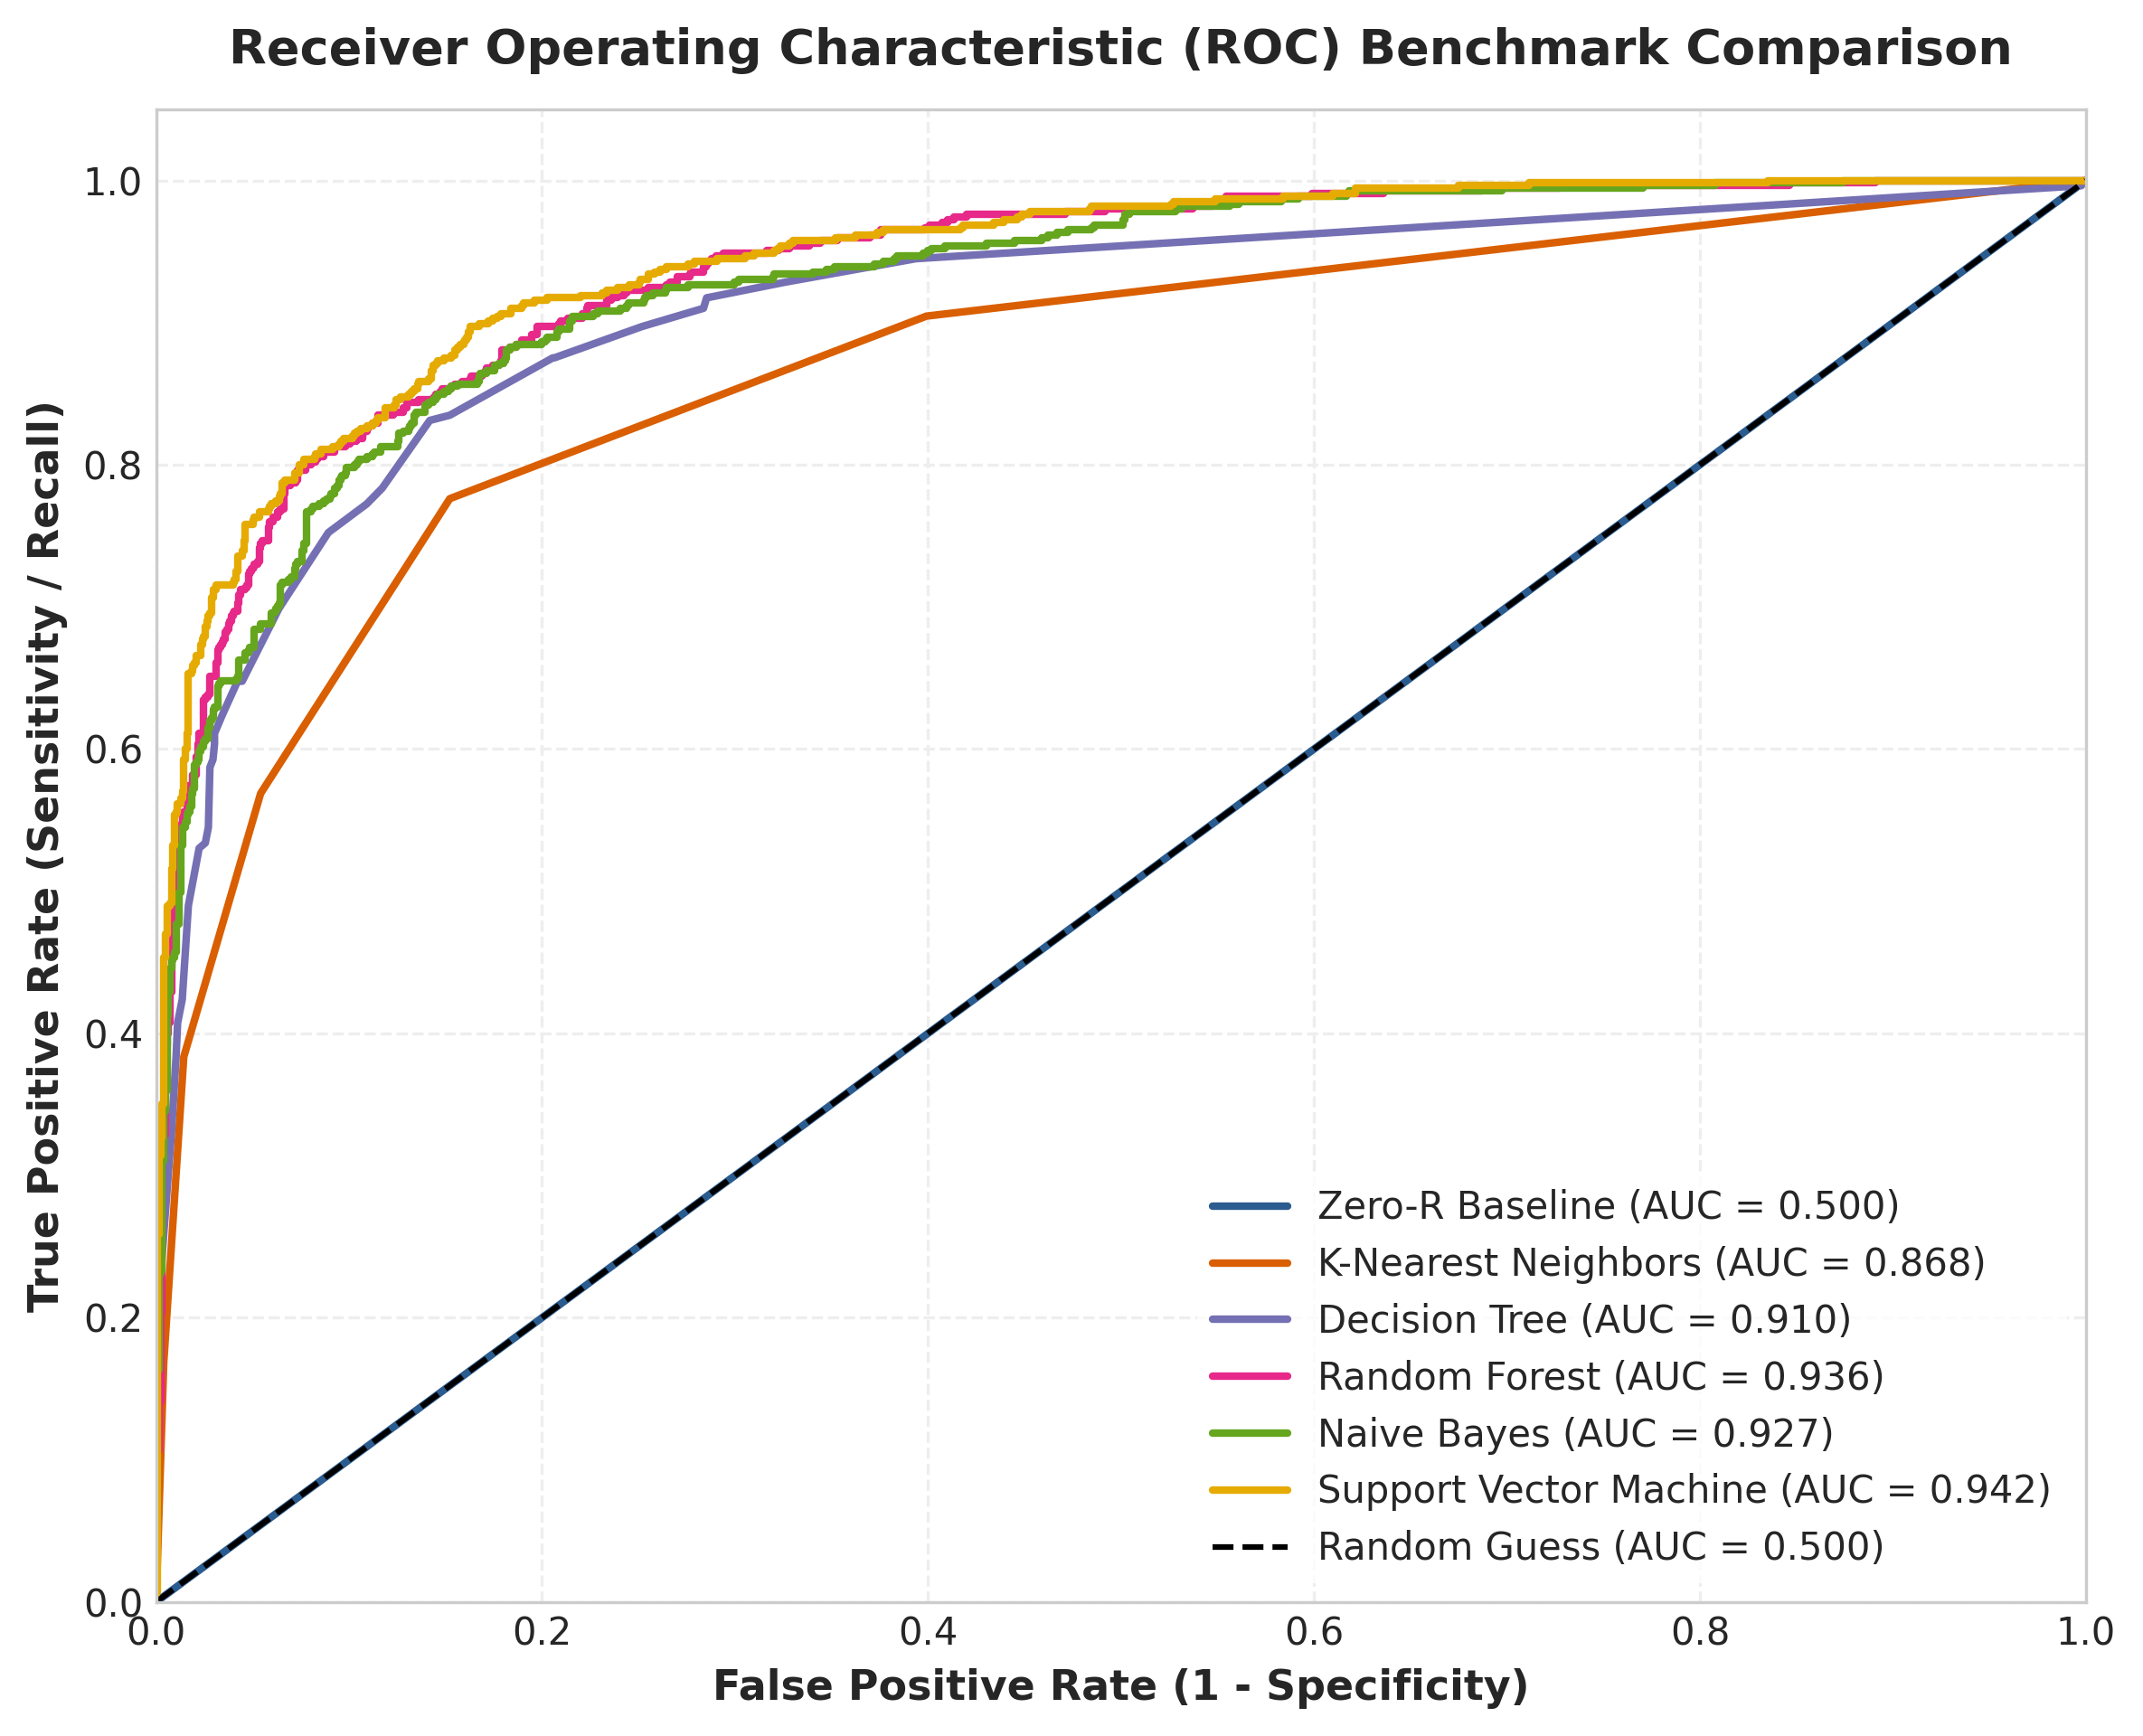
\includegraphics[width=0.75\textwidth]{figures/roc_curves.png}
\caption{Comparaison des Courbes ROC (Discrimination maximale SVM AUC = 0.9422).}
\end{figure}

\begin{figure}[H]
\centering
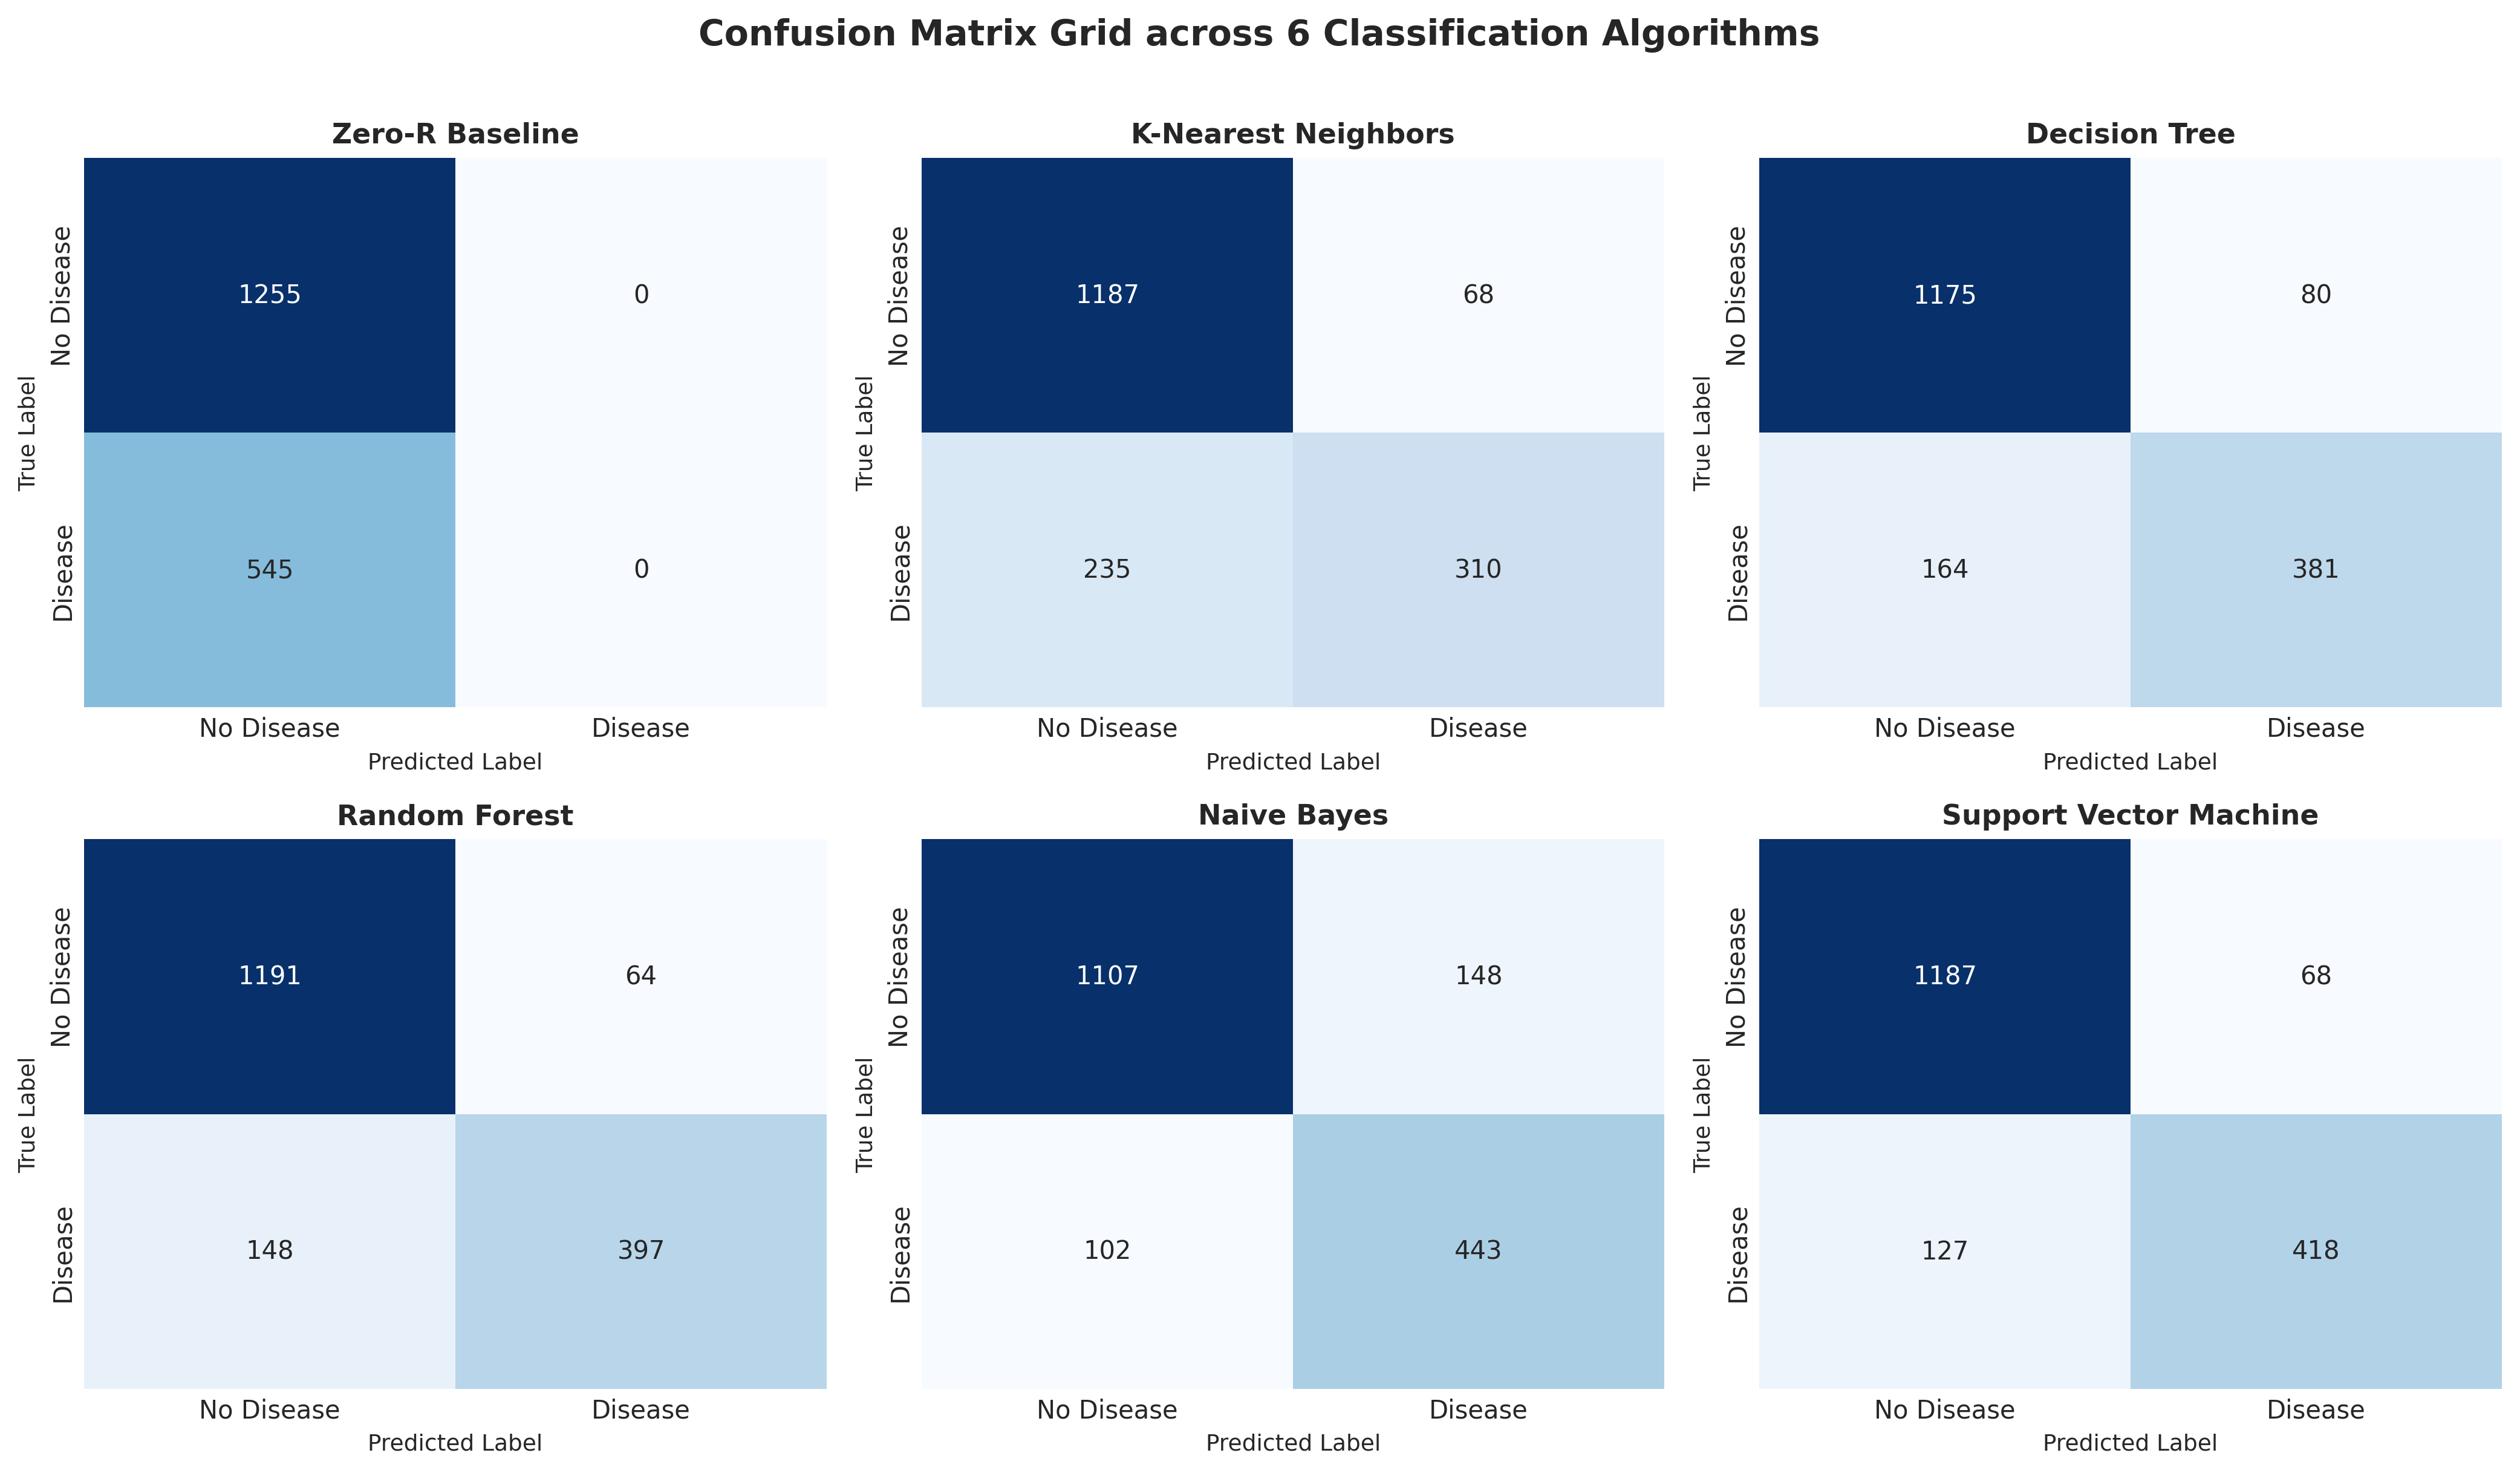
\includegraphics[width=0.82\textwidth]{figures/confusion_matrices.png}
\caption{Grille des Matrices de Confusion des 6 Algorithmes Benchmarqués.}
\end{figure}

\begin{figure}[H]
\centering
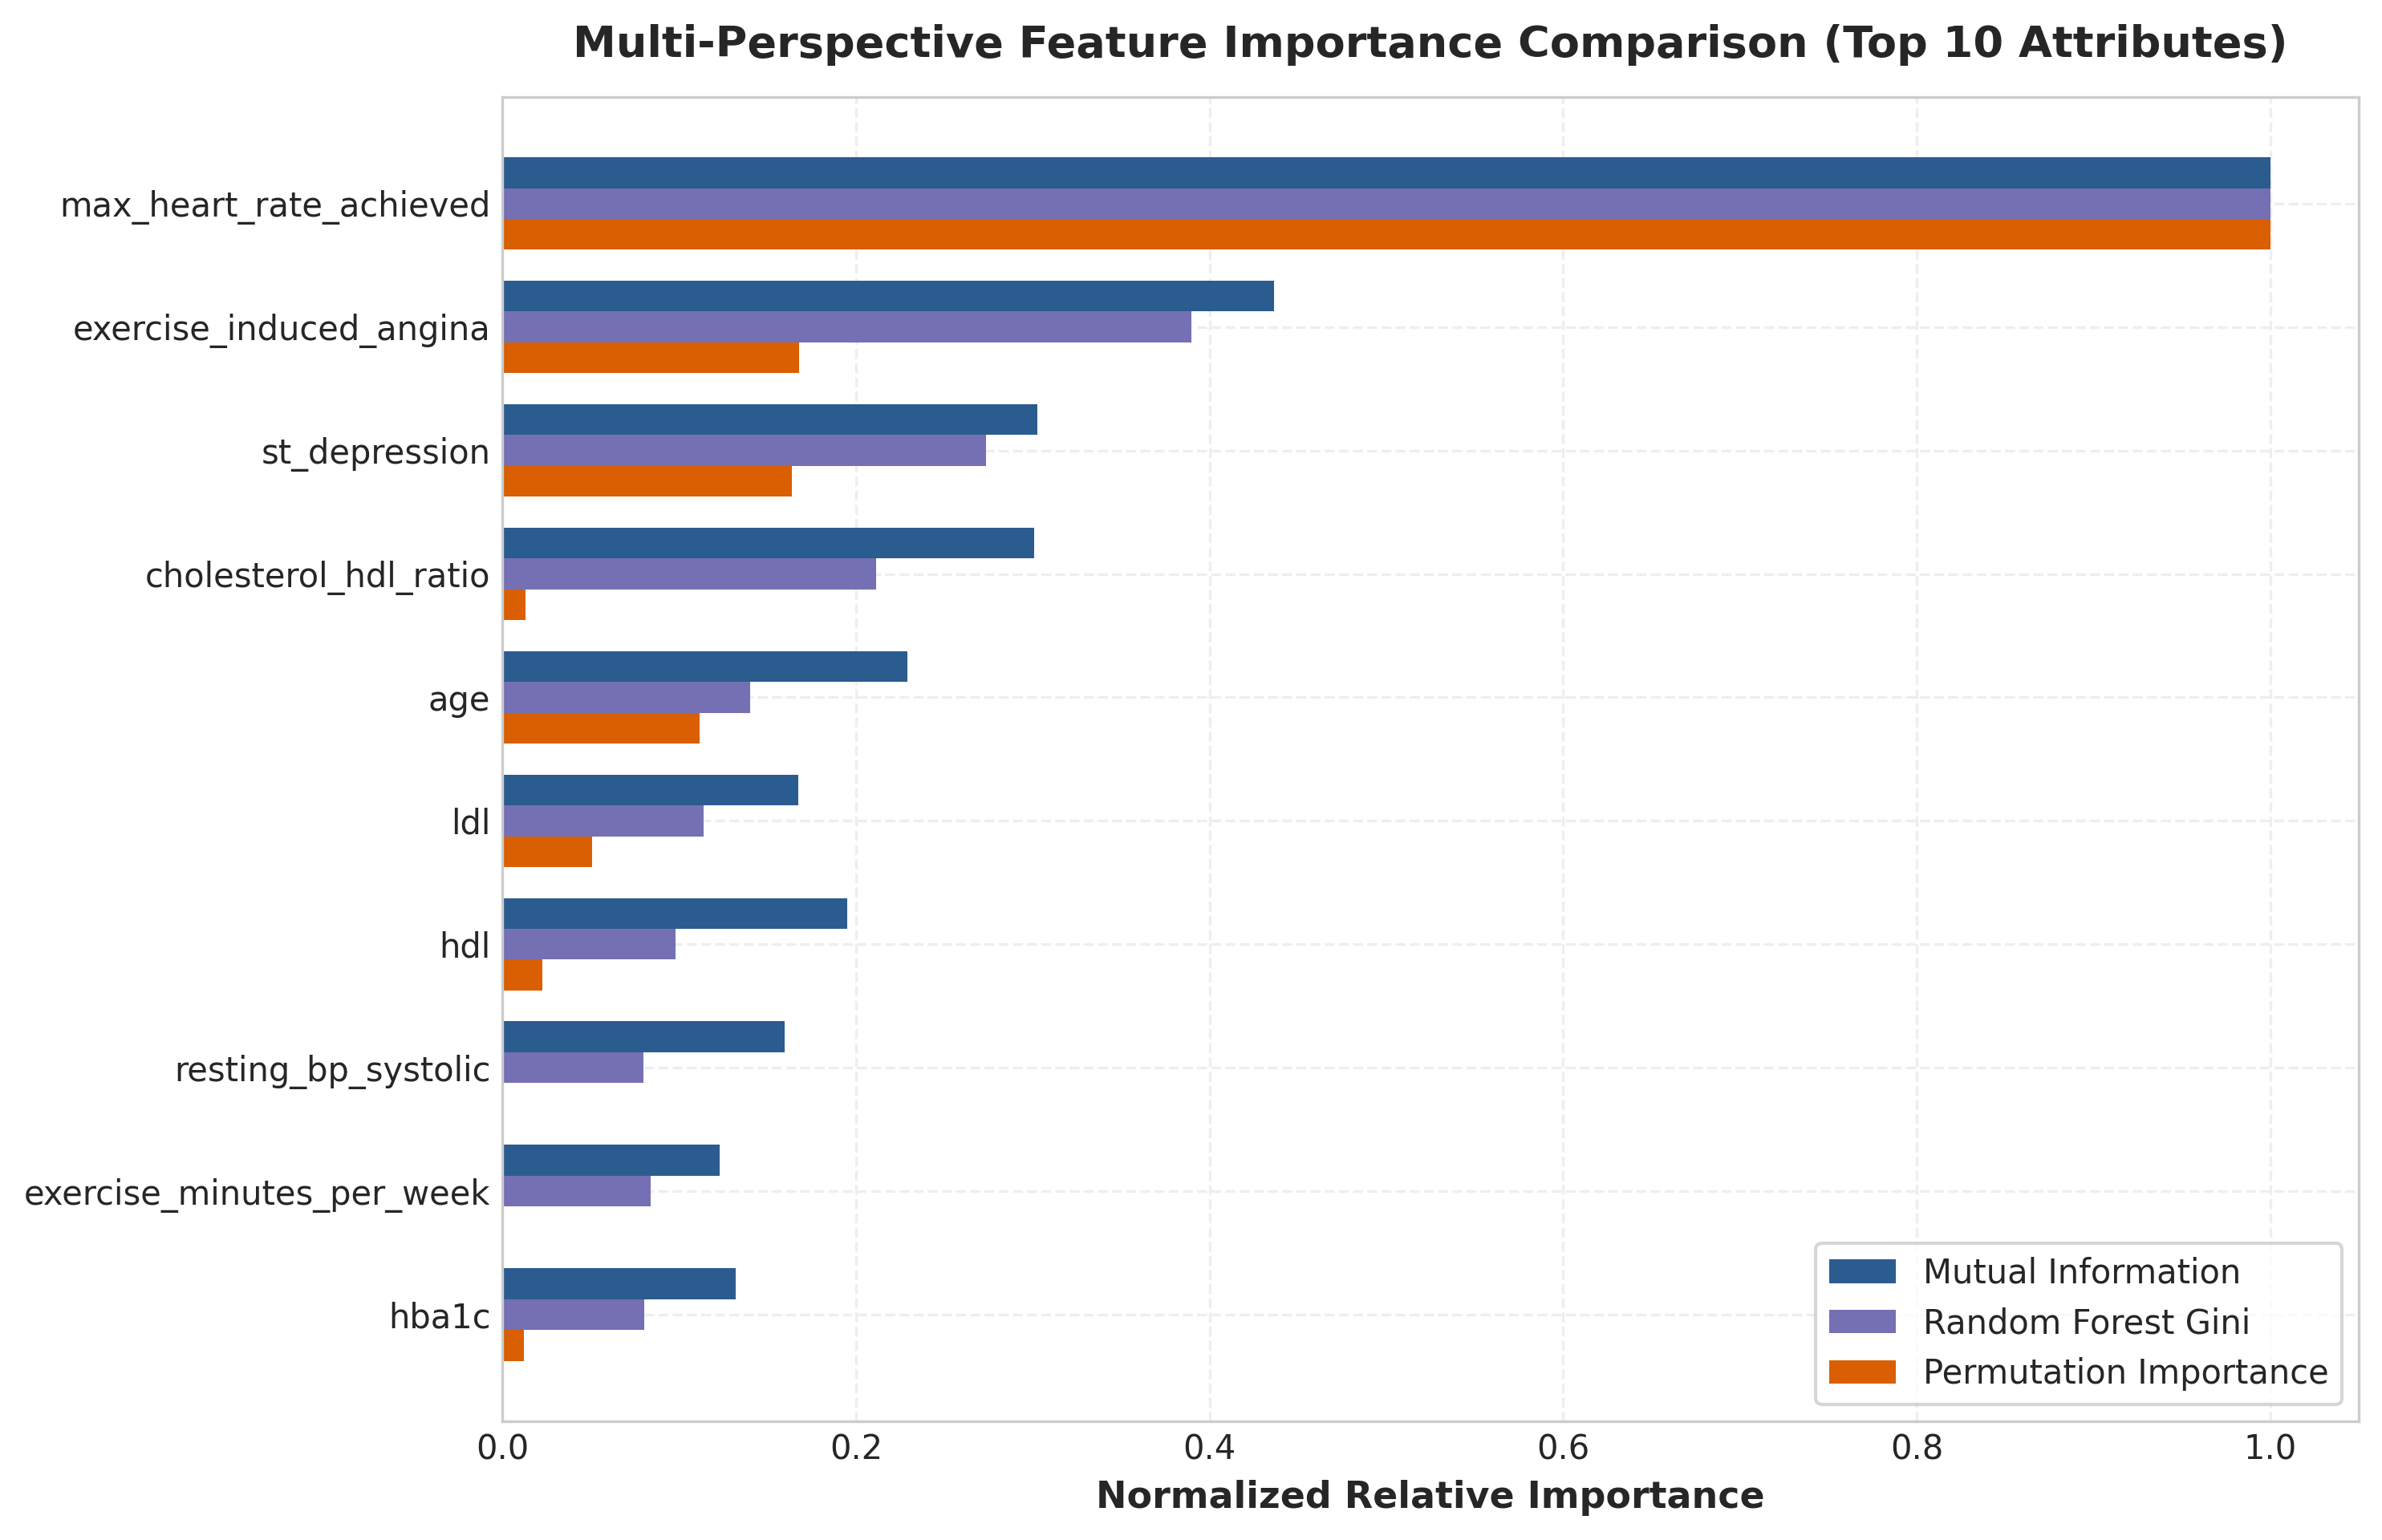
\includegraphics[width=0.82\textwidth]{figures/feature_importance_comp.png}
\caption{Analyse Multi-Perspective des Variables Clés (Fréquence Cardiaque Max, Dépression ST, Âge, LDL).}
\end{figure}

%--------------------------------------------------------------------------
\section{Modalités de Communication, Suivi et Directives Obligatoires par Email}
%--------------------------------------------------------------------------

\begin{tcolorbox}[
    colback=sintefblue!8,
    colframe=sintefblue,
    title=\textbf{DIRECTIVES OFFICIELLES DE COMMUNICATION, DE SUIVI ET DE RENDU},
    arc=2mm,
    boxrule=0.8pt,
    breakable
]

\textbf{Principe général.}

Afin de garantir une communication centralisée, une traçabilité complète des échanges
et un suivi équitable de l'avancement des différents groupes, l'ensemble des
communications officielles relatives au projet de Data Mining doit obligatoirement
être effectué par l'intermédiaire de l'adresse email officielle du projet :

\begin{center}
    \Large
    \textbf{\url{datamining.project.student@gmail.com}}
\end{center}

\textbf{Important :} les communications officielles doivent être envoyées
\textbf{exclusivement par le chef de groupe (\textit{Team Leader})}.
Les membres d'un groupe peuvent participer à la préparation du contenu du message,
mais le \textit{Team Leader} demeure le responsable de l'envoi et du suivi des
échanges avec l'équipe pédagogique.

\vspace{2mm}

Pour faciliter l'identification automatique des messages et assurer leur classement,
chaque email doit respecter strictement le format d'objet correspondant à sa nature.
Tout email ne respectant pas les conventions définies ci-dessous pourra être
retardé dans son traitement ou nécessiter une nouvelle soumission correctement
formatée.

%--------------------------------------------------------------------------
\subsection*{1. Cycle officiel de communication}

Les échanges relatifs au projet sont organisés autour de trois étapes principales :

\begin{enumerate}[leftmargin=*]

    %----------------------------------------------------------------------
    \item \textbf{Étape 1 -- Déclaration obligatoire de l'équipe et du sujet}

    \textbf{Date limite : 15 septembre 2026}

    Avant le \textbf{15 septembre 2026}, chaque \textit{Team Leader} doit envoyer
    un email officiel permettant d'enregistrer définitivement son groupe et son
    sujet de projet.

    \vspace{1mm}

    \textbf{Destinataire obligatoire :}

    \begin{center}
        \texttt{datamining.project.student@gmail.com}
    \end{center}

    \textbf{Format obligatoire de l'objet :}

    \begin{center}
        \texttt{[DM-2026][INSCRIPTION] Groupe <Code\_Leader> - <Nom\_du\_Projet>}
    \end{center}

    \textbf{Exemple :}

    \begin{center}
        \texttt{[DM-2026][INSCRIPTION] Groupe IASD01 - Prédiction Risque Cardiaque}
    \end{center}

    \textbf{Le corps de l'email doit obligatoirement contenir :}

    \begin{itemize}
        \item le code étudiant du \textit{Team Leader} ;
        \item les codes étudiants de tous les membres du groupe ;
        \item le nom ou titre provisoire du projet ;
        \item le domaine métier ou domaine d'application ;
        \item une description claire du problème à résoudre ;
        \item une description du ou des datasets envisagés ;
        \item la source du dataset et, lorsque cela est possible, son URL ;
        \item le nombre approximatif d'observations et de variables ;
        \item la variable cible (\textit{target}) envisagée, lorsqu'elle est déjà connue ;
        \item le lien vers le dépôt \textbf{GitHub public} du projet.
    \end{itemize}

    \textbf{Exemple de liste des membres :}

    \begin{center}
        \texttt{IASD01 -- Team Leader}\\
        \texttt{IASD02 -- Member}\\
        \texttt{IASD03 -- Member}\\
        \texttt{IASD04 -- Member}
    \end{center}

    \textbf{Rôle du dépôt GitHub :}

    La fourniture du lien GitHub dès la déclaration initiale est
    \textbf{strictement obligatoire}. Le dépôt constitue l'espace officiel
    permettant de suivre l'évolution technique du projet pendant toute la
    durée du semestre.

    L'équipe pédagogique pourra notamment utiliser l'historique du dépôt pour
    observer :

    \begin{itemize}
        \item la progression générale du projet ;
        \item la fréquence et la régularité des commits ;
        \item l'évolution du code source ;
        \item la contribution individuelle des membres ;
        \item l'organisation du travail ;
        \item les modifications importantes apportées au projet ;
        \item la cohérence entre l'avancement déclaré par l'équipe et
              l'avancement réellement observable dans le dépôt.
    \end{itemize}

    \textbf{Attention :} le dépôt doit rester accessible pendant toute la durée
    du projet. La suppression, la privatisation ou le remplacement du dépôt
    sans notification préalable peut empêcher le suivi de l'équipe.

    %----------------------------------------------------------------------
    \item \textbf{Étape 2 -- Demandes de support et assistance technique}

    Cette communication peut être effectuée \textbf{à tout moment pendant le
    semestre} lorsqu'une équipe rencontre une difficulté ou nécessite une
    clarification concernant le projet.

    Les demandes peuvent notamment concerner :

    \begin{itemize}
        \item le nettoyage et le prétraitement des données ;
        \item la gestion des valeurs manquantes ;
        \item la détection et le traitement des valeurs aberrantes ;
        \item l'encodage des variables catégorielles ;
        \item la normalisation ou la standardisation ;
        \item la sélection ou l'extraction des caractéristiques ;
        \item le choix d'un algorithme de Machine Learning ;
        \item l'entraînement et l'évaluation des modèles ;
        \item les métriques d'évaluation ;
        \item l'interprétation des résultats ;
        \item la visualisation des données ;
        \item l'implémentation de l'interface Streamlit ;
        \item les problèmes liés au code ou à l'environnement d'exécution.
    \end{itemize}

    \textbf{Format obligatoire de l'objet :}

    \begin{center}
        \texttt{[DM-2026][QUESTION] Groupe <Code\_Leader> - <Sujet\_de\_la\_Question>}
    \end{center}

    \textbf{Exemple :}

    \begin{center}
        \texttt{[DM-2026][QUESTION] Groupe IASD01 - Standardisation et Encodage}
    \end{center}

    Afin de permettre un traitement efficace de la demande, le message doit
    expliquer précisément :

    \begin{enumerate}
        \item le problème rencontré ;
        \item ce qui a déjà été essayé ;
        \item le résultat obtenu ;
        \item le résultat attendu ;
        \item les messages d'erreur éventuels ;
        \item les parties pertinentes du code ;
        \item les captures d'écran utiles, lorsque nécessaire.
    \end{enumerate}

    \textbf{Mauvais exemple :}

    \begin{quote}
        ``Notre code ne marche pas. Pouvez-vous nous aider ?''
    \end{quote}

    \textbf{Bon exemple :}

    \begin{quote}
        ``Après l'application de StandardScaler sur les variables numériques,
        notre modèle SVM produit une accuracy de 0.61 alors que sans
        standardisation nous obtenons 0.78. Nous avons vérifié les valeurs
        manquantes et les types des variables. Vous trouverez ci-joint le
        résultat ainsi que l'extrait du pipeline utilisé.''
    \end{quote}

    Une question clairement formulée permet une réponse plus rapide et plus
    pertinente.

    %----------------------------------------------------------------------
    \item \textbf{Étape 3 -- Déclaration d'achèvement et déclenchement de l'évaluation}

    Lorsque l'équipe considère que son projet est \textbf{entièrement terminé},
    le \textit{Team Leader} doit envoyer un email officiel déclarant
    l'achèvement du projet.

    \textbf{Format obligatoire de l'objet :}

    \begin{center}
        \texttt{[DM-2026][RENDU-FINAL] Groupe <Code\_Leader> - <Nom\_du\_Projet>}
    \end{center}

    \textbf{Exemple :}

    \begin{center}
        \texttt{[DM-2026][RENDU-FINAL] Groupe IASD01 - Prédiction Risque Cardiaque}
    \end{center}

    Cet email constitue la \textbf{déclaration officielle de fin des travaux}.
    Il indique que l'équipe considère son projet suffisamment complet pour être
    soumis à l'évaluation finale.

    Le message doit notamment confirmer :

    \begin{itemize}
        \item que tous les membres du groupe ont participé au projet ;
        \item que le dépôt GitHub contient la version finale du projet ;
        \item que le code source est accessible ;
        \item que les données et/ou liens vers les données nécessaires sont
              correctement documentés ;
        \item que le notebook ou les scripts d'analyse sont disponibles ;
        \item que les modèles finaux ont été entraînés et évalués ;
        \item que les résultats finaux sont documentés ;
        \item que l'application Streamlit, lorsqu'elle est requise, est
              fonctionnelle ;
        \item que la documentation du projet est complète.
    \end{itemize}

    %----------------------------------------------------------------------
\end{enumerate}

%--------------------------------------------------------------------------
\subsection*{2. Règles obligatoires concernant les objets des emails}

Les objets des emails constituent une partie essentielle du système de suivi.
Ils doivent être reproduits \textbf{exactement} selon les formats définis.

\begin{center}
\begin{tabular}{|p{3.2cm}|p{9cm}|}
\hline
\textbf{Type} & \textbf{Format obligatoire} \\
\hline
Inscription &
\texttt{[DM-2026][INSCRIPTION] Groupe <Code\_Leader> - <Projet>} \\
\hline
Question &
\texttt{[DM-2026][QUESTION] Groupe <Code\_Leader> - <Sujet>} \\
\hline
Rendu final &
\texttt{[DM-2026][RENDU-FINAL] Groupe <Code\_Leader> - <Projet>} \\
\hline
\end{tabular}
\end{center}

\vspace{2mm}

Les éléments suivants doivent être évités :

\begin{itemize}
    \item supprimer les balises \texttt{[DM-2026]} ;
    \item modifier les mots \texttt{INSCRIPTION}, \texttt{QUESTION} ou
          \texttt{RENDU-FINAL} ;
    \item utiliser uniquement un objet générique tel que
          ``Projet Data Mining'' ;
    \item envoyer une demande importante sans identifier le groupe ;
    \item utiliser plusieurs formats différents pour un même type de demande.
\end{itemize}

%--------------------------------------------------------------------------
\subsection*{3. Continuité et traçabilité des échanges}

Pour chaque demande concernant un même problème, il est fortement recommandé
de \textbf{répondre au même fil de discussion} plutôt que de créer plusieurs
nouveaux emails.

Cette pratique permet de conserver :

\begin{itemize}
    \item l'historique de la demande ;
    \item les réponses précédentes ;
    \item les fichiers et captures associés ;
    \item les décisions prises ;
    \item les clarifications fournies par l'équipe pédagogique.
\end{itemize}

Les équipes sont donc invitées à conserver une organisation cohérente de leurs
échanges avec l'équipe pédagogique.

%--------------------------------------------------------------------------
\subsection*{4. Conditions de prise en compte du rendu final}

L'envoi de l'email \texttt{[RENDU-FINAL]} ne signifie pas automatiquement que
le projet est conforme à toutes les exigences pédagogiques.

Il constitue la \textbf{notification officielle de disponibilité du projet
pour évaluation}.

Avant l'envoi de cet email, le \textit{Team Leader} doit donc vérifier que :

\begin{itemize}
    \item le dépôt GitHub correspond bien à la version finale ;
    \item les fichiers nécessaires sont présents ;
    \item le code peut être exécuté ;
    \item les résultats présentés correspondent aux résultats réellement obtenus ;
    \item les expériences et évaluations sont documentées ;
    \item les membres du groupe sont correctement identifiés ;
    \item les éventuelles consignes spécifiques du projet ont été respectées.
\end{itemize}

Une fois le \texttt{[RENDU-FINAL]} envoyé, toute modification importante du
projet doit être signalée à l'équipe pédagogique afin d'éviter toute ambiguïté
sur la version effectivement soumise.

%--------------------------------------------------------------------------
\subsection*{5. Déclenchement de l'évaluation}

L'email portant l'objet :

\begin{center}
    \texttt{[DM-2026][RENDU-FINAL]}
\end{center}

déclenche le processus d'évaluation du projet.

L'évaluation porte sur l'ensemble du travail réalisé par le groupe et conduit
à l'attribution de la \textbf{note finale sur 20,0 points}, conformément à la
grille d'évaluation du projet.

L'évaluation peut notamment prendre en compte :

\begin{itemize}
    \item la compréhension et la formulation du problème ;
    \item la qualité et la pertinence des données utilisées ;
    \item la qualité du prétraitement ;
    \item la méthodologie de Data Mining adoptée ;
    \item la pertinence des modèles utilisés ;
    \item la qualité des expérimentations ;
    \item l'analyse et l'interprétation des résultats ;
    \item la qualité du code ;
    \item la qualité de l'application ou de l'interface ;
    \item la documentation ;
    \item l'organisation du dépôt GitHub ;
    \item la progression et la contribution des membres observables dans
          l'historique du projet.
\end{itemize}

\end{tcolorbox}

%--------------------------------------------------------------------------
\subsection*{Résumé de la procédure}
%--------------------------------------------------------------------------

\begin{center}
\begin{tcolorbox}[
    width=0.92\textwidth,
    colback=gray!5,
    colframe=gray!60,
    title=\textbf{PROCÉDURE À SUIVRE},
    arc=2mm
]

\begin{enumerate}[leftmargin=*]
    \item \textbf{Avant le 15/09/2026 :}
    envoyer \texttt{[DM-2026][INSCRIPTION]} avec les informations du groupe,
    du sujet, du dataset et le lien GitHub.

    \item \textbf{Pendant le projet :}
    utiliser \texttt{[DM-2026][QUESTION]} pour toute demande officielle
    d’assistance ou de clarification.

    \item \textbf{Pendant toute la durée du projet :}
    maintenir le dépôt GitHub accessible et régulièrement mis à jour afin de
    permettre le suivi de l'avancement.

    \item \textbf{À la fin du projet :}
    vérifier l'ensemble des éléments du projet et publier la version finale
    sur GitHub.

    \item \textbf{Déclaration finale :}
    envoyer \texttt{[DM-2026][RENDU-FINAL]} pour déclarer officiellement
    que le projet est prêt pour l'évaluation.

    \item \textbf{Évaluation :}
    l'envoi du \texttt{[RENDU-FINAL]} déclenche le processus d'évaluation
    et l'attribution de la note finale sur 20,0 points.
\end{enumerate}

\end{tcolorbox}
\end{center}

\vspace{0.3cm}
\begin{tcolorbox}[colback=sintefgold!15, colframe=sintefgold!80!black, title=\textbf{PÉRIODE ET CALENDRIER DE SOUMISSION DES PROJETS}, arc=2mm]
    \centering
    \textbf{Le dépôt des projets est officiellement ouvert dès le premier jour du cours et reste accessible jusqu'à une semaine après la fin de la semaine des derniers examens du semestre.}
\end{tcolorbox}

\vspace{0.5cm}
\begin{center}
    {\color{sintefblue}\Large \bfseries Bon travail à toutes les équipes !}
\end{center}

\end{document}
